\chapter{Projektmanagement}

\section{Phasen}
Das Projekt erfolgt in verschiedenen Projektphasen. Da es sich um ein Forschungsprojekt handelt, wird ein iteratives Vorgehensmodell einem Wasserfallmodell vorgezogen. Aus diesem Grund werden die im Folgenden beschriebenen Phasen iterativ wiederholt.

\subsection{Evaluation/Planung}
\subsubsection{Evaluation}
Da f\"ur das CRF Projekt viel Evaluation, in der Richtung: "`Was ist \"uberhaupt m\"oglich?"', "`Welche Techniken sind die geeignetsten?"' (siehe Scene Graph Evaluation) oder "`Was gibt es bereits?"', betrieben werden muss, stellt die Evaluation einen grossen Teil des CRF Projektes dar. 

\subsubsection{Planung}
Erst wenn gewisse Erkenntnisse aus der Evaluation gewonnen werden konnten, ist es m\"oglich eine seri\"ose Planung zu erstellen. Deshalb sind diese Projektabschnitte verkn\"upft und laufen teilweise parallel.

\subsection{Design}
In der Designphase geht es haupts\"achlich darum, das Software Design f\"ur das Cave Rendering Framework zu definieren. Zum Output geh\"oren die verschiedenen Softwaredesign-Diagramme wie das Klassen- oder das Sequenzdiagramm nach UML-Standard. Der Detaillevel sollte so hoch wie m\"oglich sein und diese Modelle sollten sp\"ater nicht mehr allzugross \"andern. 

\subsection{Implementation}
In der Implementationsphase wird das CRF gem\"ass dem festgelegten Design implementiert. Ein wichtiger Teil dabei ist der parallel dazu zu entwickelnde Prototyp einer 3D Applikation, welcher das wachsende CRF nutzt und parallel dazu weiterentwickelt wird. Gegen Ende dieser Phase wird eine Demonstrator-Applikation erstellt, mit welcher s\"amtliche M\"oglichkeiten des CRF aufgezeigt und im CAVE demonstriert werden k\"onnen. Diese Applikation soll ausserdem auch f\"ur allgemeine CAVE Demonstrationen verwendet werden k\"onnen.

\subsection{Testphase}
F\"ur die Testphase werden Testcases erstellt, welche s\"amtliche verwirklichten Anforderungen und Use Cases testen und messen. Dazu geh\"oren insbesondere Funktions- und Performancetests. Fehler werden dokumentiert und korrigiert. Falls m\"oglich, werden Performanceverbesserungen vorgenommen.

\subsection{Einf\"uhrung}
Die CRF Demoapplikation wird im CAVE Labor so eingerichtet, dass sie von allen eingef\"uhrten Personen ohne grossen Aufwand zu Demonstrationszwecken und f\"ur Tests verwendet werden kann. Dazu werden die n\"otigen Personen geschult.\\
Das CRF ist so abgelegt und Dokumentiert, dass es von allen CPVR Mitarbeiter benutzt werden kann, um ihre eigenen Applikationen f\"ur den CAVE zu erstellen.

\section{Meilensteine}
\subsection{M1: Pflichtenheft liegt vor - bis 18.03.2009}
\subsubsection{Kriterien}
\begin{itemize}
	\item Pflichtenheft vorhanden mit:
	\subitem Ausgangslage
	\subitem Architektur
	\subitem Ziele
	\subitem Anforderungen
	\subitem Use Cases
	\subitem Projektmanagement
\end{itemize}

\subsection{M2: Prototyp entwickelt - bis 10.04.2009}
\subsubsection{Kriterien}
\begin{itemize}
\item Test Cases f\"ur jedes Feature
\item Projektsetup (Grobarchitektur)
\item zu verwendende Techniken klar definiert
\end{itemize}

\subsection{M3: Entwicklung abgeschlossen - bis 29.05.2009}
	
\subsubsection{M3.1: Designkonzept steht}
\paragraph{Kriterien}
\begin{itemize}
	\item Klassendiagramme vorhanden
	\item Sequenzdiagramme vorhanden
	\item zu verwendende Techniken klar definiert
\end{itemize}
\subsubsection{M3.2: Implementation abgeschlossen}
\paragraph{Kriterien}
\begin{itemize}
	\item Technische Dokumentation liegt vor
	\item Benutzerdokumentation liegt vor
	\item Prim\"are Use Cases implementiert 
	\item Prim\"are Anforderungen erf\"ullt
	\item Demoapplikation l\"auft
\end{itemize}
\subsubsection{M4: Testphase abgeschlossen}
\paragraph{Kriterien}
\begin{itemize}
	\item Testprotokolle liegen vor
	\item Fehler korrigiert
	\item Demoapplikationen funktionieren fehlerfrei
\end{itemize}
\subsection{M4: Dokumentation abgeschlossen - 12.06.2009}
\subsubsection{Kriterien}
\begin{itemize}
	\item Meilensteine 1-3 erfolgreich abgeschlossen
	\item Technische Dokumentation
	\item Benutzerdokumentation
	\item Projektjournal
\end{itemize}

\clearpage
\section{Projektplan}
\begin{figure}[ht]
\centering
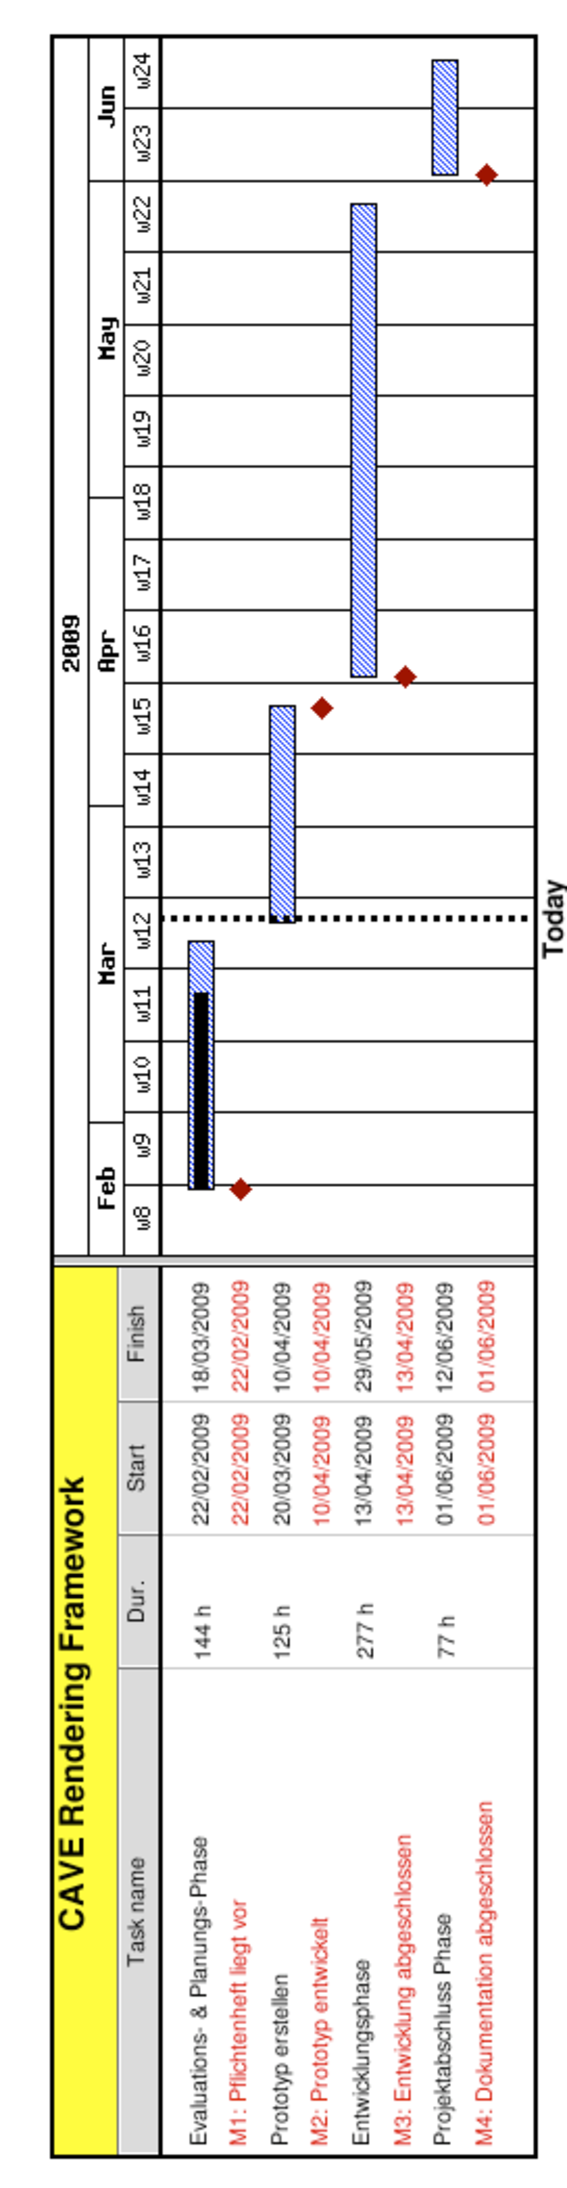
\includegraphics[scale=0.45]{../figures/gantt_20_3_09}
\caption{Projektplanung per 20.03.2009}
\end{figure}